\documentclass[tikz,border=8pt]{standalone}
\usepackage{amsmath}
\usetikzlibrary{arrows.meta,positioning,calc}

\begin{document}
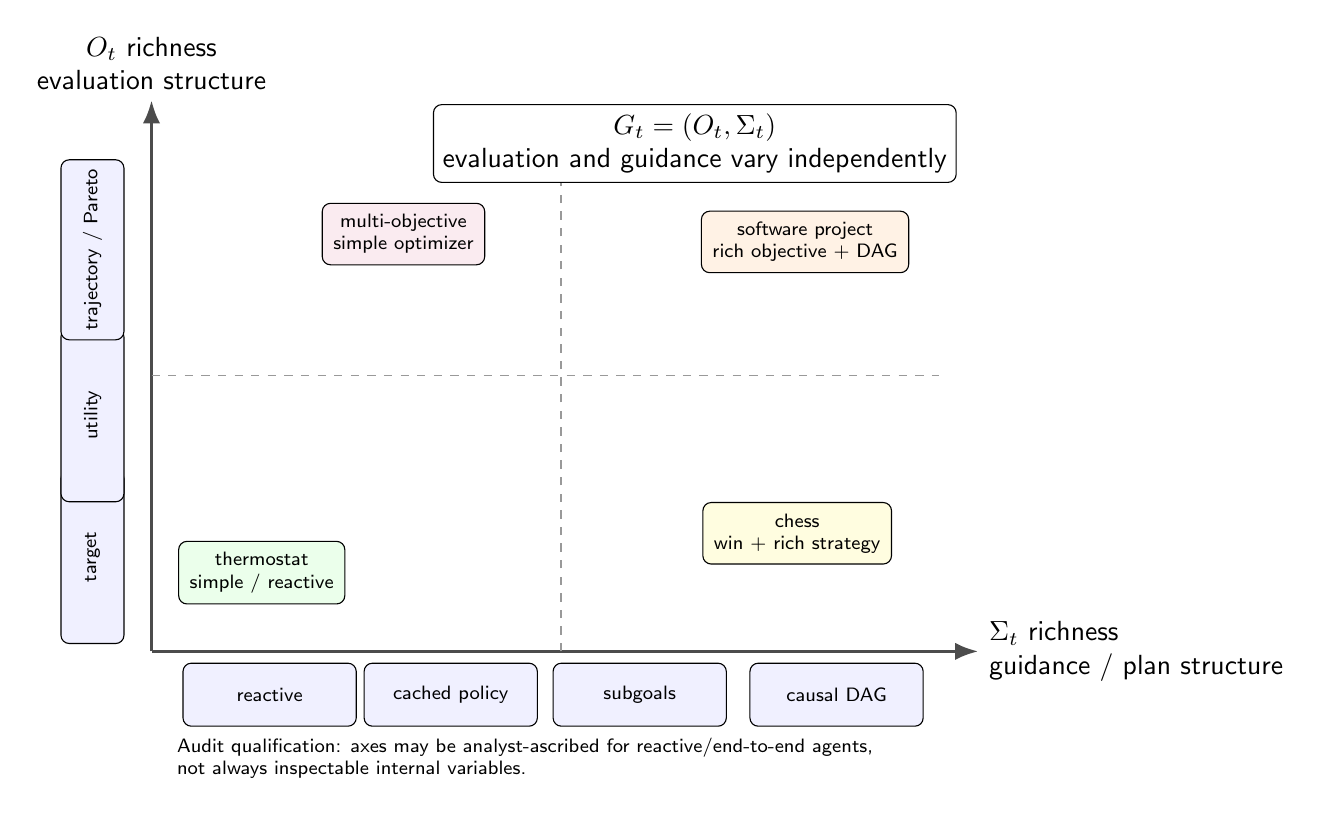
\begin{tikzpicture}[
  font=\sffamily,
  axis/.style={-Latex, very thick, draw=black!70},
  point/.style={draw, rounded corners=3pt, align=center, fill=white, inner sep=4pt, font=\sffamily\scriptsize},
  band/.style={draw, rounded corners=3pt, align=center, fill=blue!6, minimum width=22mm, minimum height=8mm, font=\sffamily\scriptsize},
  note/.style={align=center, font=\sffamily\scriptsize}
]

\coordinate (o) at (0,0);
\draw[axis] (o) -- (10.5,0) node[right, align=left] {$\Sigma_t$ richness\\guidance / plan structure};
\draw[axis] (o) -- (0,7.0) node[above, align=center] {$O_t$ richness\\evaluation structure};

\node[band] at (1.5,-0.55) {reactive};
\node[band] at (3.8,-0.55) {cached policy};
\node[band] at (6.2,-0.55) {subgoals};
\node[band] at (8.7,-0.55) {causal DAG};

\node[band, rotate=90] at (-0.75,1.2) {target};
\node[band, rotate=90] at (-0.75,3.0) {utility};
\node[band, rotate=90] at (-0.75,5.1) {trajectory / Pareto};

\node[point, fill=green!8] (thermo) at (1.4,1.0) {thermostat\\simple / reactive};
\node[point, fill=yellow!12] (chess) at (8.2,1.5) {chess\\win + rich strategy};
\node[point, fill=purple!8] (mo) at (3.2,5.3) {multi-objective\\simple optimizer};
\node[point, fill=orange!10] (project) at (8.3,5.2) {software project\\rich objective + DAG};

\draw[dashed, draw=black!40] (0,3.5) -- (10,3.5);
\draw[dashed, draw=black!40] (5.2,0) -- (5.2,6.5);

\node[draw, rounded corners=3pt, align=center, fill=white, minimum width=45mm] at (6.9,6.45)
  {$G_t=(O_t,\Sigma_t)$\\evaluation and guidance vary independently};

\node[note, align=left, anchor=west] at (0.2,-1.35)
  {Audit qualification: axes may be analyst-ascribed for reactive/end-to-end agents,\\not always inspectable internal variables.};

\end{tikzpicture}
\end{document}
